\section{Transformation rules (smoothening, scales and shifts).} \label{scales_and_shifts}
As we have seen, the Euclidean distance is efficient and easily computable but it doesn't capture similar time-series in the presence of noise, scales or shifts. Much effort have been put in to overcome this issue. As mentioned before, in \cite{citeulike:3815880} authors introduced scale and the shift shape-perceiving transformations which are applied before measuring the similarity with Euclidean distance. Their proposed definition of similar time-series is based on the transformation $T_{a,b}$ where $a$ is the scaling coefficient and $b$ is the shift coefficient. This ``similarity transformation $T_{a,b}$'' is a mapping of each of the $x_{i} \in X$ into $x_{i}\acute{} = a*x_{i}+b$ and if this transformation can be found for two time-series $X$ and $Y$ such that $X=T_{a,b}(Y)$ time-series $X$ and $Y$ are considered to be similar.

Agrawal et al. \cite{citeulike:3816327} proposed more general method of aligning of time-series by allowing any arbitrary segment of the query time-series to be scaled and stretched by any suitable amount and adding the ability of deletion of any non-matching segment (note that this work also seems to be the one of the first proposing LCS application to time-series similarity, see \ref{lcs}). Also, they introduced an $\epsilon$ envelope around the template sequence which aimed to deal with noise on the query time-series. The figure  \ref{fig:transform} shows principles of such a method walking from the raw time series through discussed transformations.

\begin{figure}[tbp]
   \centering
   \includegraphics[height=50mm]{transform.eps}
   %%{seriesheatmap}
   \caption{Illustration of scaling, smoothening and shifting: the leftmost plot depicts the raw time-series, plot at the middle shows the query time-series after scaling and smoothening and the plot at the right adds shifts to transform while showing $\epsilon$ alignment envelope.}
   \label{fig:transform}
\end{figure} 

Since the Euclidean distance is calculated only after discussed transformations applied, it is unable to capture the cost and complexity of the these transformations and does not reflect the true similarity. If the cost assigned to the each of the transformations performed \cite{citeulike:3731711}, than the integral of all effective costs will measure the true similarity between time-series.

The complexity of scales and shift transformation is $O(NM)$ where $N$ and $M$ are the query and template sequences.

